\chapter{Initial implementation}

\lstinputlisting{code/MLDU_Simple.m}

\noindent The block MLDU algorithm was implemented using MATLAB. It represents a typical first attempt without many optimizations. It uses pre-allocation for the output matrices and a nested function for the splitting of the matrix.

\section{Verification and performance analysis}

A simple test was required to verify the correctness of the implementation of the algorithm and analyze its performance. The following code was used:

\lstinputlisting{code/Test_Function_1.m}
\lstinputlisting{code/Matrix_A.m}

\vspace{5mm}

\newpage
\noindent As an example, matrix A and s are provided below ($n = 4$): 

$$
A = 
\left\lbrack\begin{array}{rrrr|rrrr|rrrr|rrrr}
           4&          -1&           0&           0&          -1&           0&           0&           0&           0&           0&           0&           0&           0&           0&           0&           0\\
          -1&           4&          -1&           0&           0&          -1&           0&           0&           0&           0&           0&           0&           0&           0&           0&           0\\
           0&          -1&           4&          -1&           0&           0&          -1&           0&           0&           0&           0&           0&           0&           0&           0&           0\\
           0&           0&          -1&           4&           0&           0&           0&          -1&           0&           0&           0&           0&           0&           0&           0&           0\\ \hline
          -1&           0&           0&           0&           4&          -1&           0&           0&          -1&           0&           0&           0&           0&           0&           0&           0\\
           0&          -1&           0&           0&          -1&           4&          -1&           0&           0&          -1&           0&           0&           0&           0&           0&           0\\
           0&           0&          -1&           0&           0&          -1&           4&          -1&           0&           0&          -1&           0&           0&           0&           0&           0\\
           0&           0&           0&          -1&           0&           0&          -1&           4&           0&           0&           0&          -1&           0&           0&           0&           0\\ \hline
           0&           0&           0&           0&          -1&           0&           0&           0&           4&          -1&           0&           0&          -1&           0&           0&           0\\
           0&           0&           0&           0&           0&          -1&           0&           0&          -1&           4&          -1&           0&           0&          -1&           0&           0\\
           0&           0&           0&           0&           0&           0&          -1&           0&           0&          -1&           4&          -1&           0&           0&          -1&           0\\
           0&           0&           0&           0&           0&           0&           0&          -1&           0&           0&          -1&           4&           0&           0&           0&          -1\\  \hline
           0&           0&           0&           0&           0&           0&           0&           0&          -1&           0&           0&           0&           4&          -1&           0&           0\\
           0&           0&           0&           0&           0&           0&           0&           0&           0&          -1&           0&           0&          -1&           4&          -1&           0\\
           0&           0&           0&           0&           0&           0&           0&           0&           0&           0&          -1&           0&           0&          -1&           4&          -1\\
           0&           0&           0&           0&           0&           0&           0&           0&           0&           0&           0&          -1&           0&           0&          -1&           4\\
\end{array}\right\rbrack
$$

$$
s =
\left\lbrack\begin{array}{rrrrrrrr}
           2&           2&           2&           2&           2&           2&           2&           2\\
\end{array}\right\rbrack
$$

\noindent Running the test with $n = 100$ creates a $10.000 \times 10.000$ matrix. Calculating the Frobenius norm of the error results in:

\vspace{5mm}

\noindent \texttt{>> [ E ] = Test\_Function\_1( 100, @MLDU\_Simple )}\\
\\
\texttt{E =}\\
\\
\texttt{   1.1409e-13}

\vspace{5mm}

\noindent The resulting error is small enough to be confident in the correct operation of the implementation, at least for this test case.

\vspace{5mm}

\noindent Running the profiler with the same input results in the following table:

\begin{figure}[h!]
    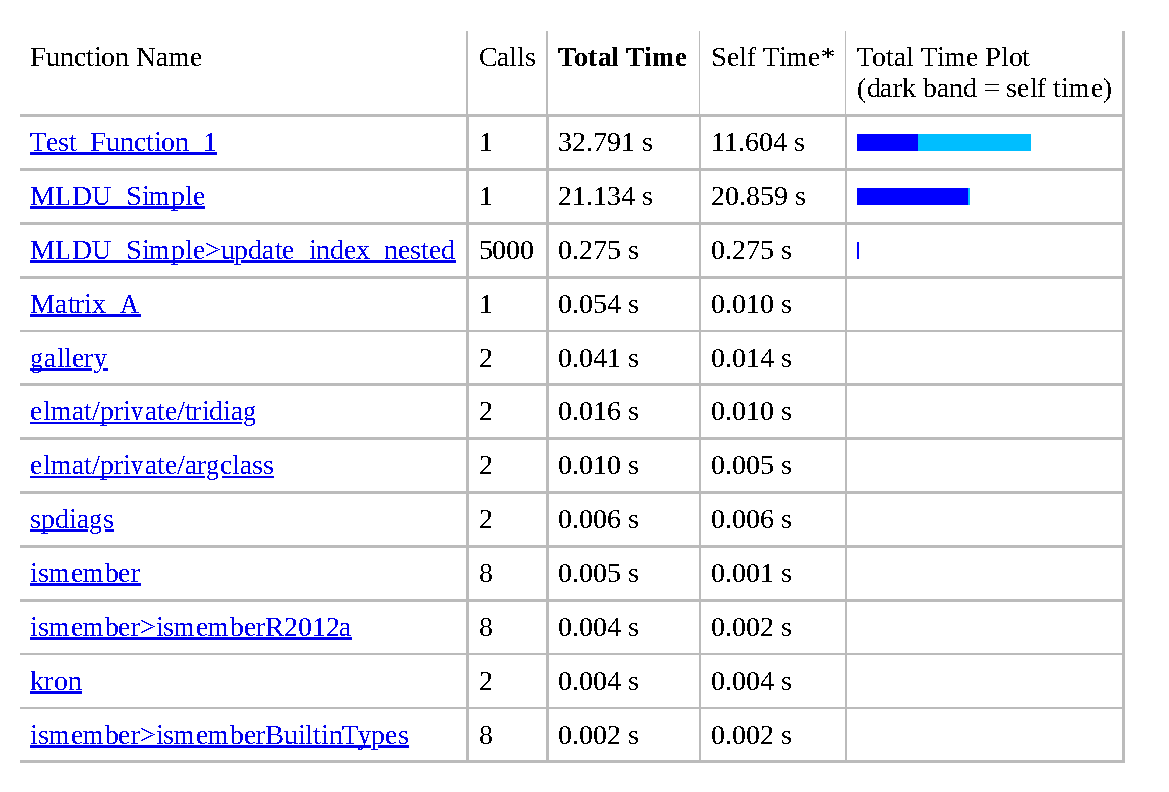
\includegraphics[width=\linewidth]{figures/Profile_MLDU_Simple_1.eps}
    \centering
\end{figure}

\noindent The first thing to note is that the runtime is about $30$ seconds for this test case, of which roughly $20$ seconds are spend by the \texttt{MLDU\_Simple} function. A $10.000 \times 10.000$ matrix is not really small, but it's not large either. As such, $20$ seconds to provide the factorization is a rather poor result.

\newpage

\noindent To get a better understanding of what is going on, the following profiler information was pulled up:

\begin{figure}[h!]
    \includegraphics[width=0.95\linewidth]{figures/Profile_MLDU_Simple_2.eps}
    \centering
\end{figure}

\noindent About 12 seconds of the runtime are spent calculating the Frobenius norm of the error, which can clearly be omitted from the performance analysis. Zooming in on the profiler information of the \texttt{MLDU\_Simple.m} function yields:

\begin{figure}[b!]
    \includegraphics[width=0.95\linewidth]{figures/Profile_MLDU_Simple_3.eps}
    \centering
    \label{Piramid}
\end{figure}

\newpage

\section{Discussion of the results}

\noindent The results mostly speak for themselves. A huge part of the runtime of the implementation is spent on line $27$, where the results of the Schur complement update gets subtracted from the matrix. Even though there are some calculations involved in this line, they could not account for this excessive runtime.\\

\noindent Calculating the Schur complement happens at lines $23$, $24$ and $25$, which takes about $1.5$ seconds. Most of that time is not actually spent doing any calculations, but rather accessing the elements of matrix \texttt{U}. This is to be expected, as the sparse storage format of MATLAB is catered towards accessing columns rather than rows. Further proof of this can be found at line $21$, where separating the elements of \texttt{U} from \texttt{A} actually takes more time than calculating the Schur complement update.\\

\noindent The point is that most of the runtime of line $27$ will most likely be spent on the memory operations associated with inserting columns and rows of data into an existing sparse matrix. There are a couple of obvious possibilities that might be tried to circumvent this problem:

\begin{itemize}
    \item Switch from sparse to full matrix storage.
    \item Store rows in a transposed fashion.
    \item Use a matrix storage format that doesn't require as many memory operations to insert rows and columns.
\end{itemize}

\noindent The first possibility may seem silly, but is not as stupid as may at first appear. Fill-in is a real nemesis of algorithms like Block MLDU, and can make a sparse matrix very full in some instances. Switching to full matrix storage in these situations makes perfect sense and will provide a very healthy performance improvement.\\

\noindent Storing the rows as transposed columns can have tangible benefits, but it has certain disadvantages as well. The most obvious downside is the extra memory consumption, as the matrix will probably need to be stored twice. The second problem is that the block nature of the algorithm makes a lot of the work required to adapt the code that much harder.\\
\noindent It should be noted that this possible improvement should definitely be investigated further, as it could be a huge advantage in situations where the input matrix is symmetric.\\

\noindent Switching to a different matrix storage format will probably provide the most benefits, especially if the storage format is designed from scratch and tailored to the needs of the Block MLDU algorithm. The second implementation of the algorithm will focus on this possibility.
